\documentclass[svgnames,11pt]{beamer}
\input{/home/tof/Documents/Cozy/latex-include/preambule_commun.tex}
\input{/home/tof/Documents/Cozy/latex-include/preambule_beamer.tex}
%\usepackage{pgfpages} \setbeameroption{show notes on second screen=left}
\author[]{Christophe Viroulaud}
\title{Véhicule autonome - suivre un tracé}
\date{}
%\logo{}
\institute{Seconde - SNT}
\usepackage{tikz}
\usetikzlibrary{shapes}
\begin{document}
\begin{frame}
\titlepage
\end{frame}


\section{Problématique}
\begin{frame}
    \frametitle{Problématique}

    Un véhicule autonome doit pouvoir utiliser les informations extérieures pour adapter son comportement. Typiquement, il peut repérer les lignes blanches pour garder un positionnement correct sur la route.
\begin{center}
\centering
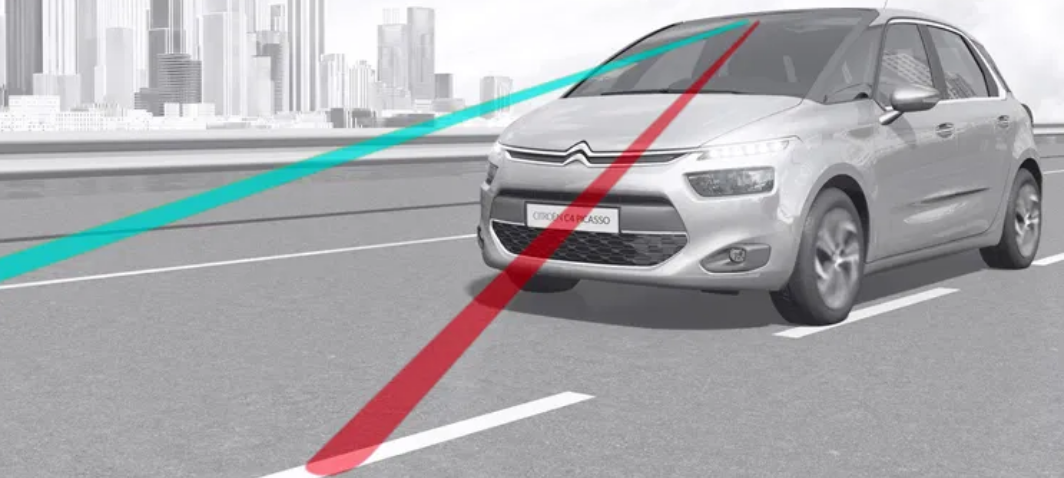
\includegraphics[width=6cm]{ressources/lignes.png}
\captionof{figure}{Repérer les lignes blanches}
\label{lignes}
\end{center}

\end{frame}

\begin{frame}
    \frametitle{}

    \begin{center}
        \framebox{Comment programmer un robot pour qu'il suive un tracé?}
    \end{center}

\end{frame}
\begin{frame}
    \frametitle{}

    \begin{activite}
    Construire une fiche bilan de l'activité réalisée aujourd'hui. Elle comprendra:
    \begin{itemize}
        \item la problématique abordée,
        \item les réflexions sur l'algorithme:
        \begin{itemize}
            \item les propositions pour répondre à la problématique (questionnement du groupe),
            \item les réflexions et les solutions sur les différents points de difficultés,
        \end{itemize}
        \item l'implémentation (le codage):
        \begin{itemize}
            \item les instructions utilisables,
            \item les codes implémentés dans le robot pour répondre à la problématique.
        \end{itemize}
    \end{itemize}
    La présentation est libre. La clarté du cheminement réalisé, des explications prendra une part non négligeable dans la note.
    \end{activite}
\note[item]{Premier temps seul à partir d'ici, puis présentation de \emph{Réfléchir à l'algorithme}}
\end{frame}
\section{Réfléchir à l'algorithme}
\begin{frame}
    \frametitle{Réfléchir à l'algorithme}
    
\begin{aretenir}[Question]
Comment peut-on repérer la trace au sol?
\end{aretenir}
    

\end{frame}
\begin{frame}
    \frametitle{Correction}

    Sous le robot, il y a deux capteurs de sol.
    \begin{center}
    \centering
    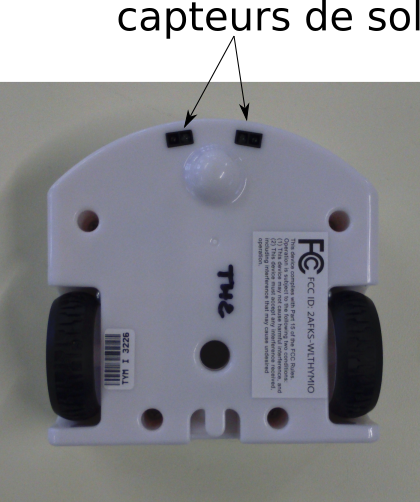
\includegraphics[width=6cm]{ressources/capteurs-sol.png}
    \captionof{figure}{Capteurs}
    \label{capteurs}
    \end{center}

\end{frame}
\begin{frame}
    \frametitle{}

    \begin{aretenir}[Question]
    Quelle logique mettre en place pour que le robot suive la trace noire?
    \end{aretenir}

\end{frame}
\begin{frame}
    \frametitle{Correction}

    Il faut utiliser les deux capteurs indépendamment.

\end{frame}
\begin{frame}
    \frametitle{}

    \begin{center}
    \centering
    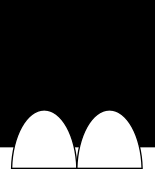
\includegraphics[width=7cm]{ressources/diode1.png}
    \captionof{figure}{Si les deux capteurs repèrent le noir: \textbf{avancer}}
    \label{IMG}
    \end{center}

\end{frame}
\begin{frame}
    \frametitle{}

    \begin{center}
    \centering
    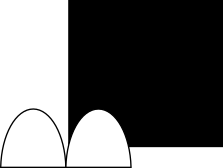
\includegraphics[width=8cm]{ressources/diode2.png}
    \captionof{figure}{Si la diode gauche repère le blanc: \textbf{tourner à droite}}
    \label{IMG}
    \end{center}

\end{frame}
\begin{frame}
    \frametitle{}

    \begin{center}
    \centering
    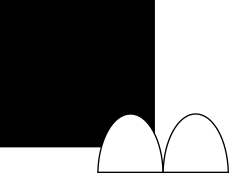
\includegraphics[width=8cm]{ressources/diode3.png}
    \captionof{figure}{Si la diode droite repère le blanc: \textbf{tourner à gauche}}
    \label{IMG}
    \end{center}

\end{frame}
\begin{frame}
    \frametitle{}

    \begin{aretenir}[Question]
    Quelle logique mettre alors en place?
    \end{aretenir}

\end{frame}
\begin{frame}
    \frametitle{Logigramme}

    \begin{center}
    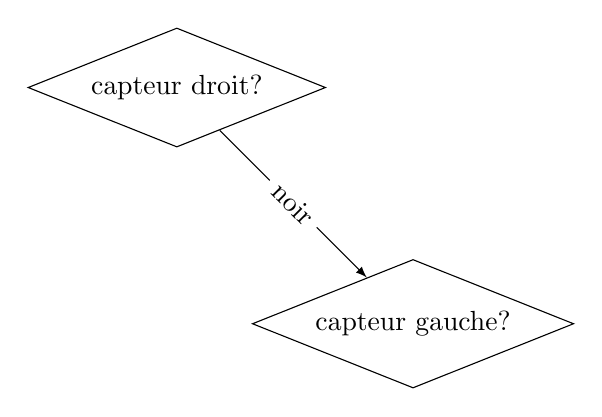
\begin{tikzpicture}
    \node[draw,diamond,aspect=2.5] (A) at (0,0){capteur droit?};
    \node[draw,diamond,aspect=2.5] (C) at (3,-3){capteur gauche?};

    \draw[->,>=latex] (A)--(C) node[sloped, midway, fill=white]{noir};
    \end{tikzpicture}
    \end{center}

\end{frame}
\begin{frame}
    \frametitle{Logigramme}

    \begin{center}
    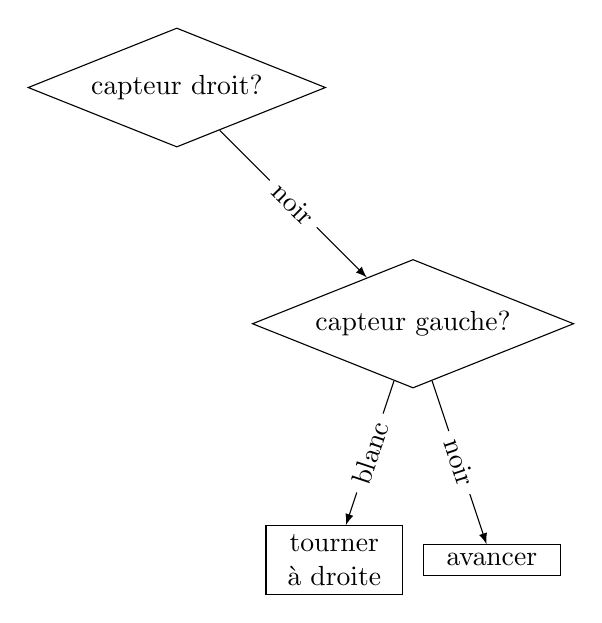
\begin{tikzpicture}
    \node[draw,diamond,aspect=2.5] (A) at (0,0){capteur droit?};
    \node[draw,diamond,aspect=2.5] (C) at (3,-3){capteur gauche?};
    \node[draw,text width=1.5cm,text centered] (F) at (2,-6){tourner à droite};
    \node[draw,text width=1.5cm,text centered] (G) at (4,-6){avancer};

    \draw[->,>=latex] (A)--(C) node[sloped, midway, fill=white]{noir};
    \draw[->,>=latex] (C)--(F) node[sloped, midway, fill=white]{blanc};
    \draw[->,>=latex] (C)--(G) node[sloped, midway, fill=white]{noir};
    \end{tikzpicture}
    \end{center}

\end{frame}
\begin{frame}
    \frametitle{Logigramme}

    \begin{center}
    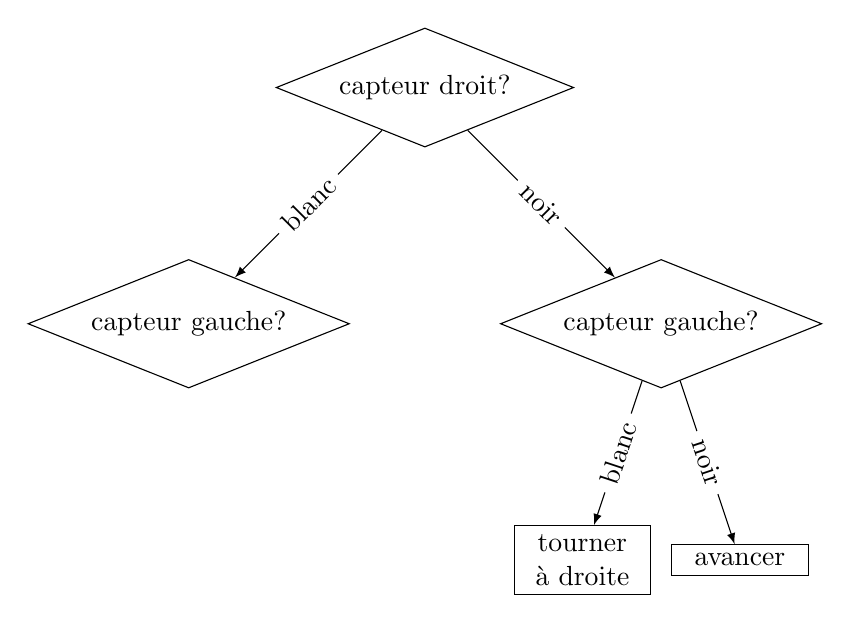
\begin{tikzpicture}
    \node[draw,diamond,aspect=2.5] (A) at (0,0){capteur droit?};
    \node[draw,diamond,aspect=2.5] (B) at (-3,-3){capteur gauche?};
    \node[draw,diamond,aspect=2.5] (C) at (3,-3){capteur gauche?};
    \node[draw,text width=1.5cm,text centered] (F) at (2,-6){tourner à droite};
    \node[draw,text width=1.5cm,text centered] (G) at (4,-6){avancer};

    \draw[->,>=latex] (A)--(B) node[sloped, midway, fill=white]{blanc};
    \draw[->,>=latex] (A)--(C) node[sloped, midway, fill=white]{noir};
    \draw[->,>=latex] (C)--(F) node[sloped, midway, fill=white]{blanc};
    \draw[->,>=latex] (C)--(G) node[sloped, midway, fill=white]{noir};
    \end{tikzpicture}
    \end{center}

\end{frame}
\begin{frame}
    \frametitle{Logigramme}

    \begin{center}
    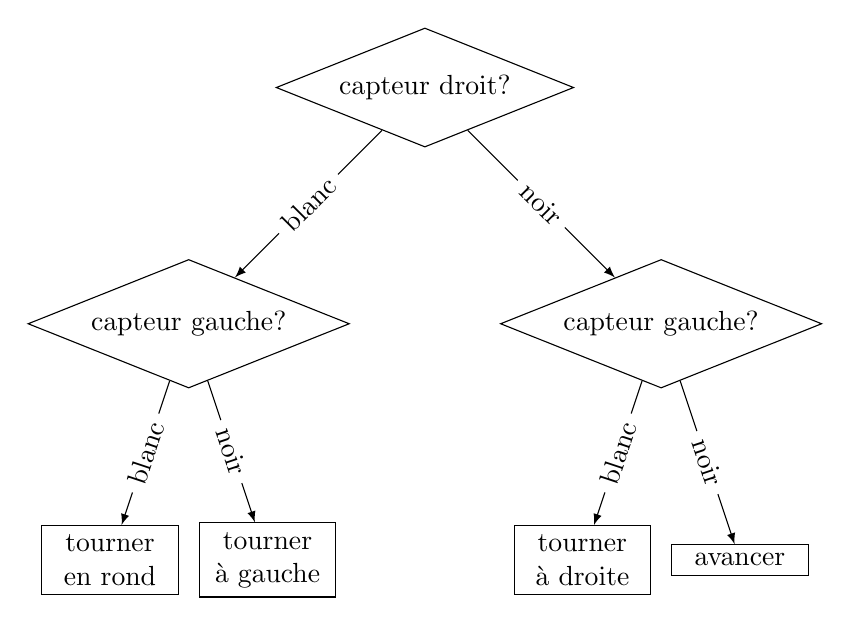
\begin{tikzpicture}
    \node[draw,diamond,aspect=2.5] (A) at (0,0){capteur droit?};
    \node[draw,diamond,aspect=2.5] (B) at (-3,-3){capteur gauche?};
    \node[draw,diamond,aspect=2.5] (C) at (3,-3){capteur gauche?};
    \node[draw,text width=1.5cm,text centered] (D) at (-4,-6){tourner en rond};
    \node[draw,text width=1.5cm,text centered] (E) at (-2,-6){tourner à gauche};
    \node[draw,text width=1.5cm,text centered] (F) at (2,-6){tourner à droite};
    \node[draw,text width=1.5cm,text centered] (G) at (4,-6){avancer};

    \draw[->,>=latex] (A)--(B) node[sloped, midway, fill=white]{blanc};
    \draw[->,>=latex] (A)--(C) node[sloped, midway, fill=white]{noir};
    \draw[->,>=latex] (B)--(D) node[sloped, midway, fill=white]{blanc};
    \draw[->,>=latex] (B)--(E) node[sloped, midway, fill=white]{noir};
    \draw[->,>=latex] (C)--(F) node[sloped, midway, fill=white]{blanc};
    \draw[->,>=latex] (C)--(G) node[sloped, midway, fill=white]{noir};
    \end{tikzpicture}
    \end{center}
\note[item]{tourner en rond = comportement du programme cyan}
\note[item]{\textbf{Le code est exécuté en boucle: attend qu'un événement se déclenche.}}
\end{frame}
\section{Implémenter l'algorithme}
\begin{frame}
    \frametitle{Implémenter l'algorithme}
\begin{aretenir}[Question]
De quelles instructions disposons-nous?
\end{aretenir}
\begin{activite}
Tester les instructions:
\begin{itemize}
    \item Tourner dans le sens horaire.
    \item Tourner à droite.
\end{itemize}
Quelle différence constate-t-on entre ces deux instructions?
\end{activite}

\end{frame}
\begin{frame}
    \frametitle{}

    \begin{aretenir}[Question]
    Écrire le code reprenant le logigramme.
    \end{aretenir}
\note[item]{programmation événementielle}
\note[item]{Il faudra peut-être adapter les vitesses.}
\end{frame}
\begin{frame}
    \frametitle{Initialisation}

    \begin{center}
    \centering
    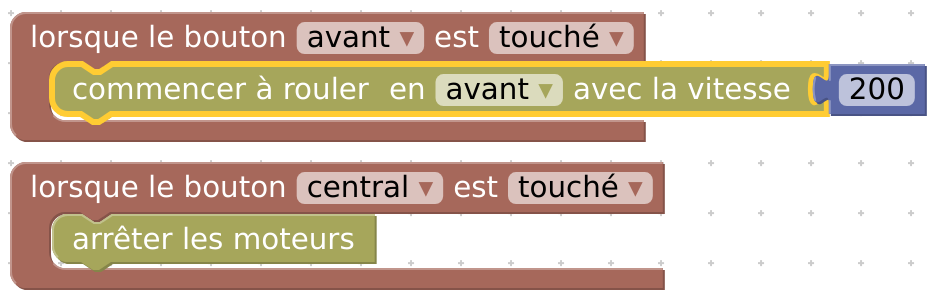
\includegraphics[width=11cm]{ressources/init.png}
    \end{center}

\end{frame}
\begin{frame}
    \frametitle{Capteur gauche}

    \begin{center}
    \centering
    
\includegraphics[width=11cm]{ressources/gauche.png}
    \end{center}

\end{frame}
\begin{frame}
    \frametitle{Capteur droit}

    \begin{center}
    \centering
    
\includegraphics[width=11cm]{ressources/droite.png}
    \end{center}

\end{frame}

\end{document}